\documentclass[../notes.tex]{subfiles}
\graphicspath{{\subfix{../img/}}}
\begin{document}

\section{Goals of Control Theory}
Control theory is a branch of engineering that deals with the behavior of dynamical systems and how to influence that behavior through inputs. Typical considerations are:
\begin{description}
    \item[Stability] Ensuring the system remains bounded and predictable over time, and preventing oscillations or otherwise chaotic behavior.
    \item[Controllability] Determining whether a system can be driven from an initial state to a desired final state using the available control inputs.
    \item[Observability] Assessing how much of the internal state of a system can be inferred from its outputs. Crucial for systems where direct measurement of all variables isn't possible.
    \item[Optimality] Achieving the desired behavior with minimal cost (energy, time). Involves balancing between speed, accuracy, and resource usage.
    \item[Robustness] Maintaining performance despite uncertainties, disturbances, or modelling inaccuracies. The controller must be able to handle real world imperfections!
    % \item[Feedback Design] Correcting errors and adapting to changes
\end{description}

\begin{figure}[H]
    \centering
    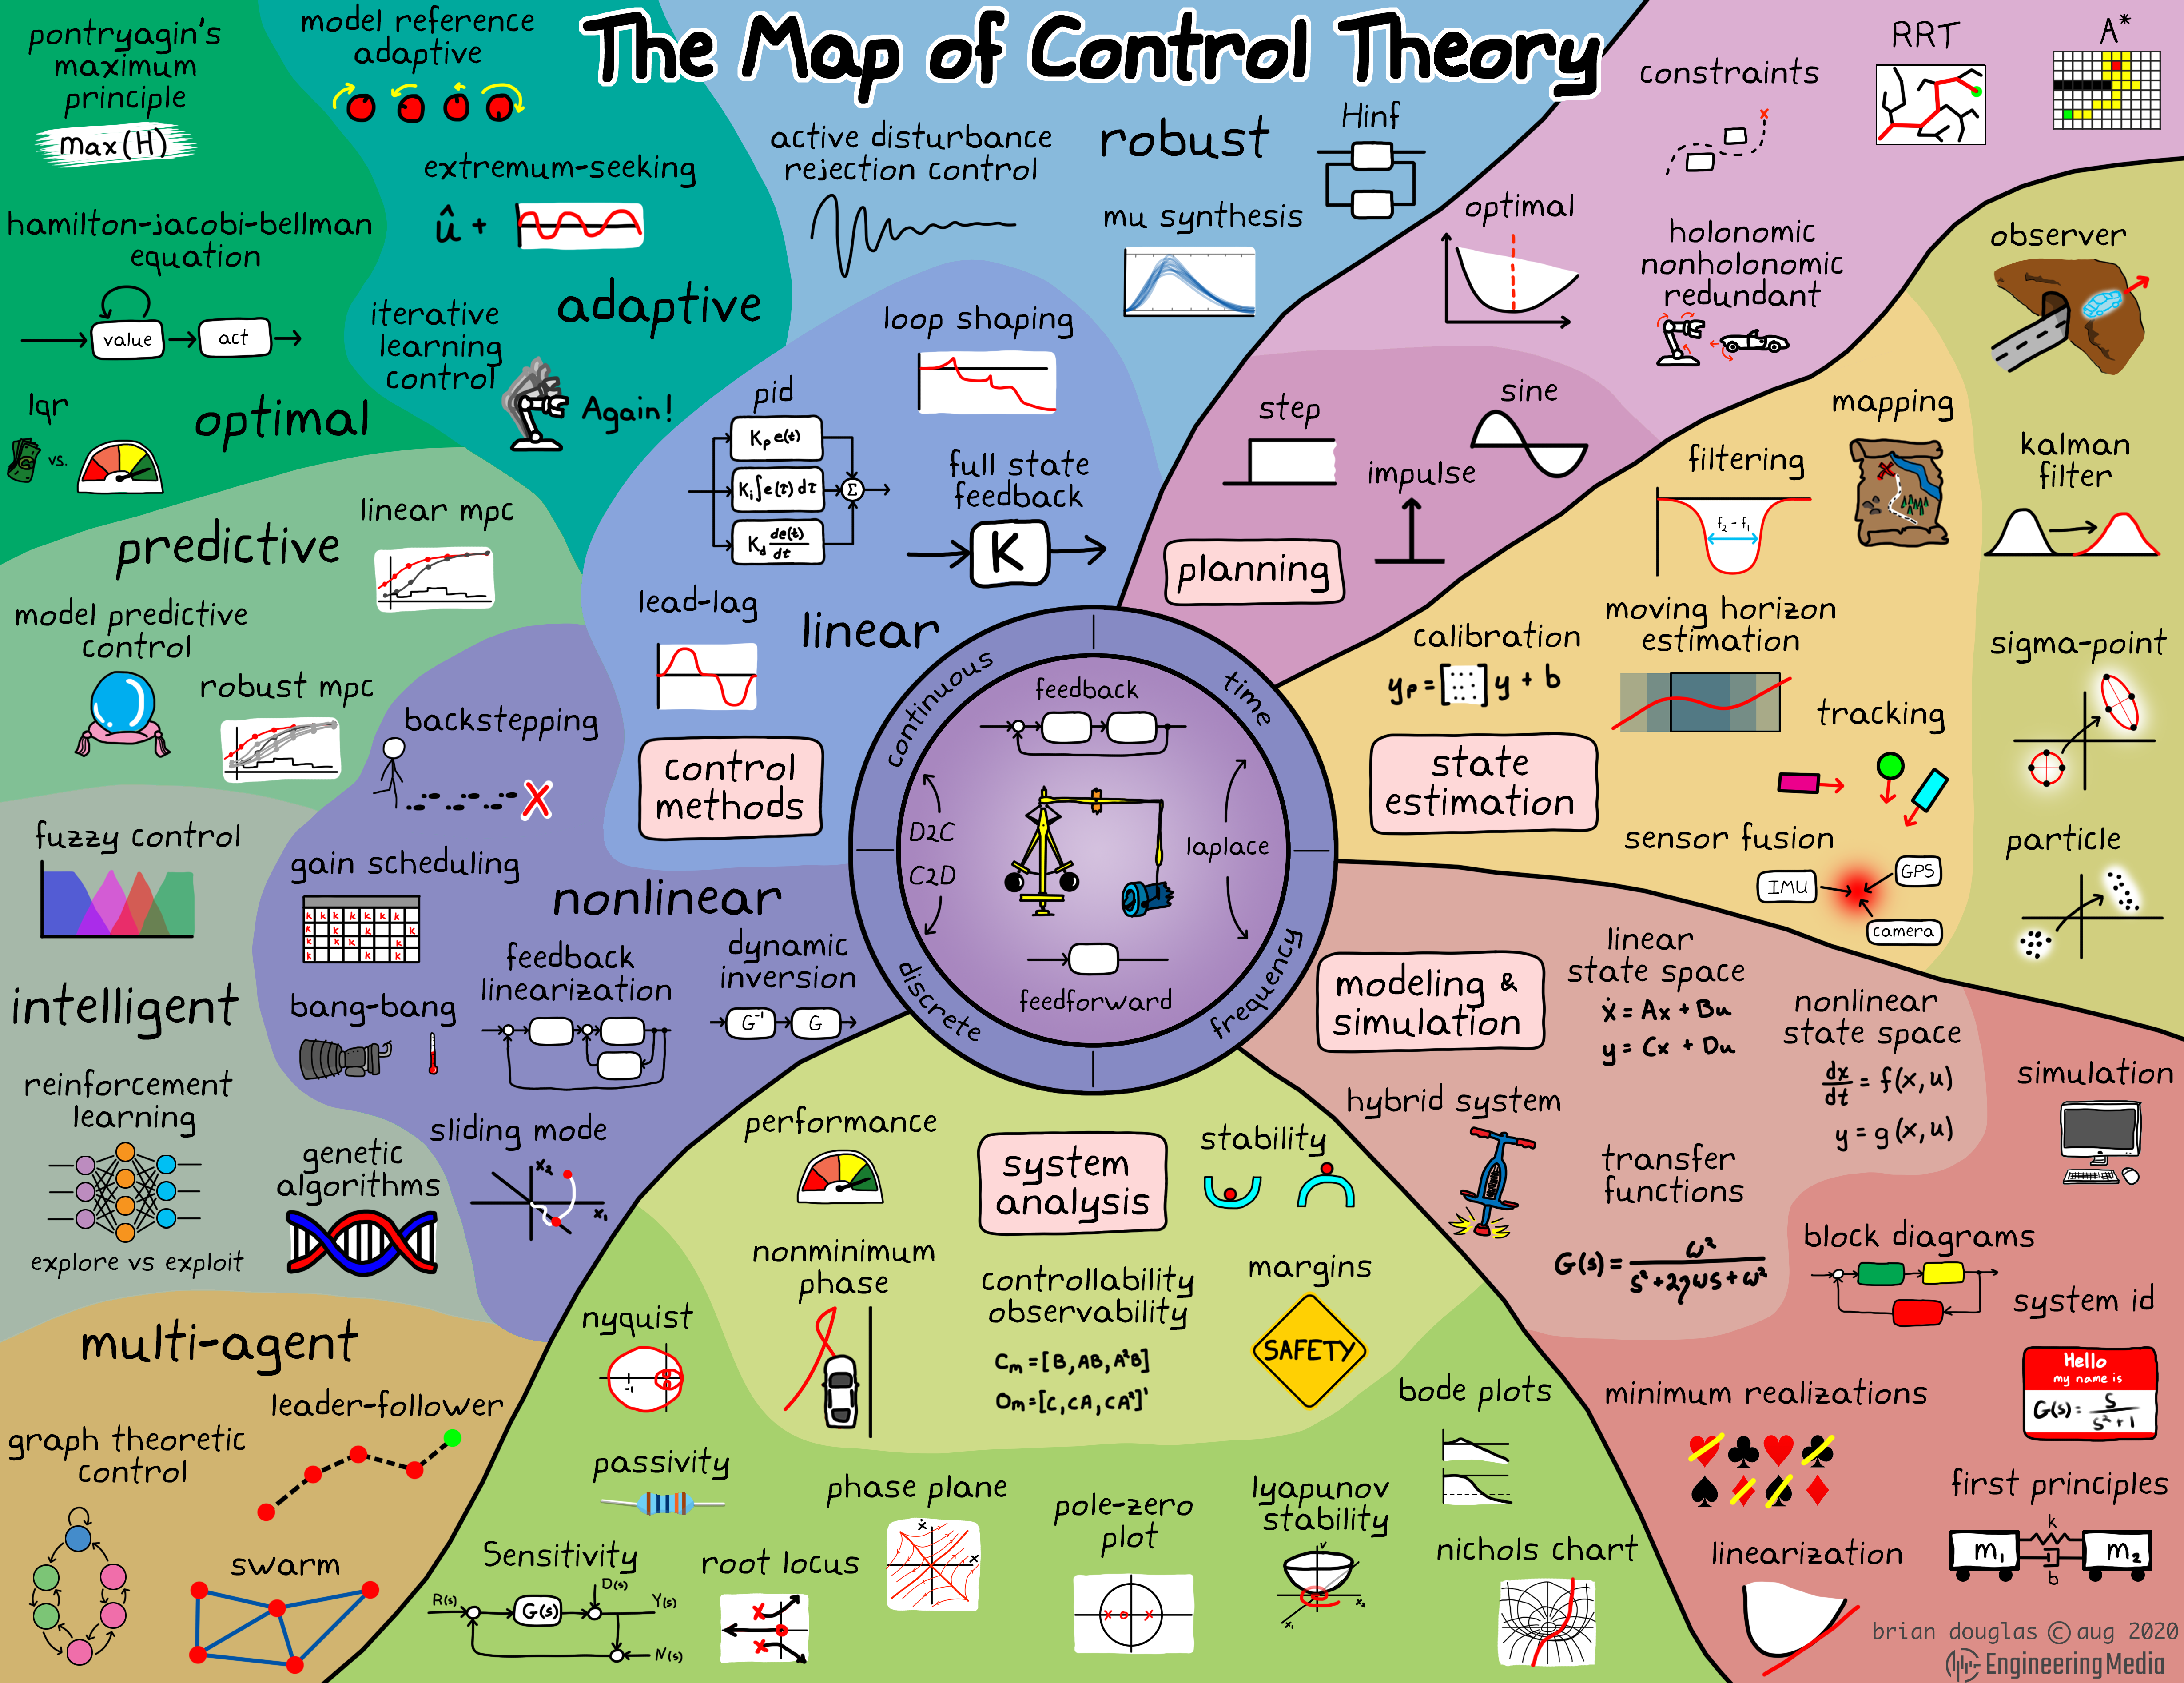
\includegraphics[width=1\linewidth]{Control_Map.png}
    \caption{Brian Douglas' Concept Map of Control Theory}
    \label{fig:controlMap}
\end{figure}

Control theory is a interdisciplinary topic. It can be applied to mechanical, electrical, thermal, fluid, really any system.

\subsection{Applications to Aerospace}
The main application of control theory in aerospace is in Guidance, Navigation, and Control (GNC). In order from most broad to least:
\begin{description}
    \item[Navigation] "Given the measurements we have, where do we think we are?"
    \item[Guidance] "Given where we want to go and where we think we are, which path should we follow?"
    \item[Control] "What effort should we apply and how should we control actuators given where we are and the chosen path?"
\end{description}
These can be further broken down into numerous subcategories.\\ 
Control theory offers many benefits in the aerospace application. 
\begin{description}
    \item[Automation]
    \item[Performance]
    \item[Safeguards / Protections]
    \item[Deferred Decision-making]    
\end{description}

\end{document}